\chapter{Dataset, Methodology and Experimental Setup}\label{ch:method}

\section{SeizeIT2 Dataset}

SeizeIT2 \cite{bhagubai2025seizeit2} (OpenNeuro ds005873 v1.1.0, CC0) holds wearable recordings of 125 patients with
focal epilepsy from five European epilepsy units, with seizures annotated on hospital video-EEG. We use the official
split: \textbf{96 training patients} for all development and \textbf{29 test patients} scored once, after the design
was frozen. Tables~\ref{tab:modalities} and~\ref{tab:inventory} and Figures~\ref{fig:classes} and~\ref{fig:hours}
summarise it (all values measured by our audit).

\begin{table}[H]
\centering\small
\caption{Signals recorded by the wearable (rates measured from the files).}\label{tab:modalities}
\begin{tabular}{@{}llc@{}}
\toprule
\textbf{Signal} & \textbf{Channels} & \textbf{Rate}\\
\midrule
Behind-the-ear EEG & 2 (left, right or cross-head) & 256 Hz\\
ECG & 1 & 256 Hz\\
EMG & 1 & 256 Hz\\
Motion & 3-axis accelerometer + 3-axis gyroscope & 25 Hz\\
\bottomrule
\end{tabular}
\end{table}

\begin{table}[H]
\centering\small
\caption{Inventory of SeizeIT2 measured by our audit.}\label{tab:inventory}
\begin{tabular}{@{}ll@{}}
\toprule
\textbf{Quantity} & \textbf{Value}\\
\midrule
Patients / recordings / EDF files & 125 / 2,850 / 11,009 (125.9 GB)\\
Hours of EEG & 11,626 h (median 95 h per patient)\\
Seizures & 883 (train 702, test 181)\\
Seizure time & 14.3 h = \textbf{0.123\,\%} of the recording time\\
Seizure duration & 2--962 s (median 33 s)\\
Missing ECG/EMG; missing motion & 3.1\,\%; 3.9\,\% of the time\\
\bottomrule
\end{tabular}
\end{table}

\begin{figure}[H]
\centering
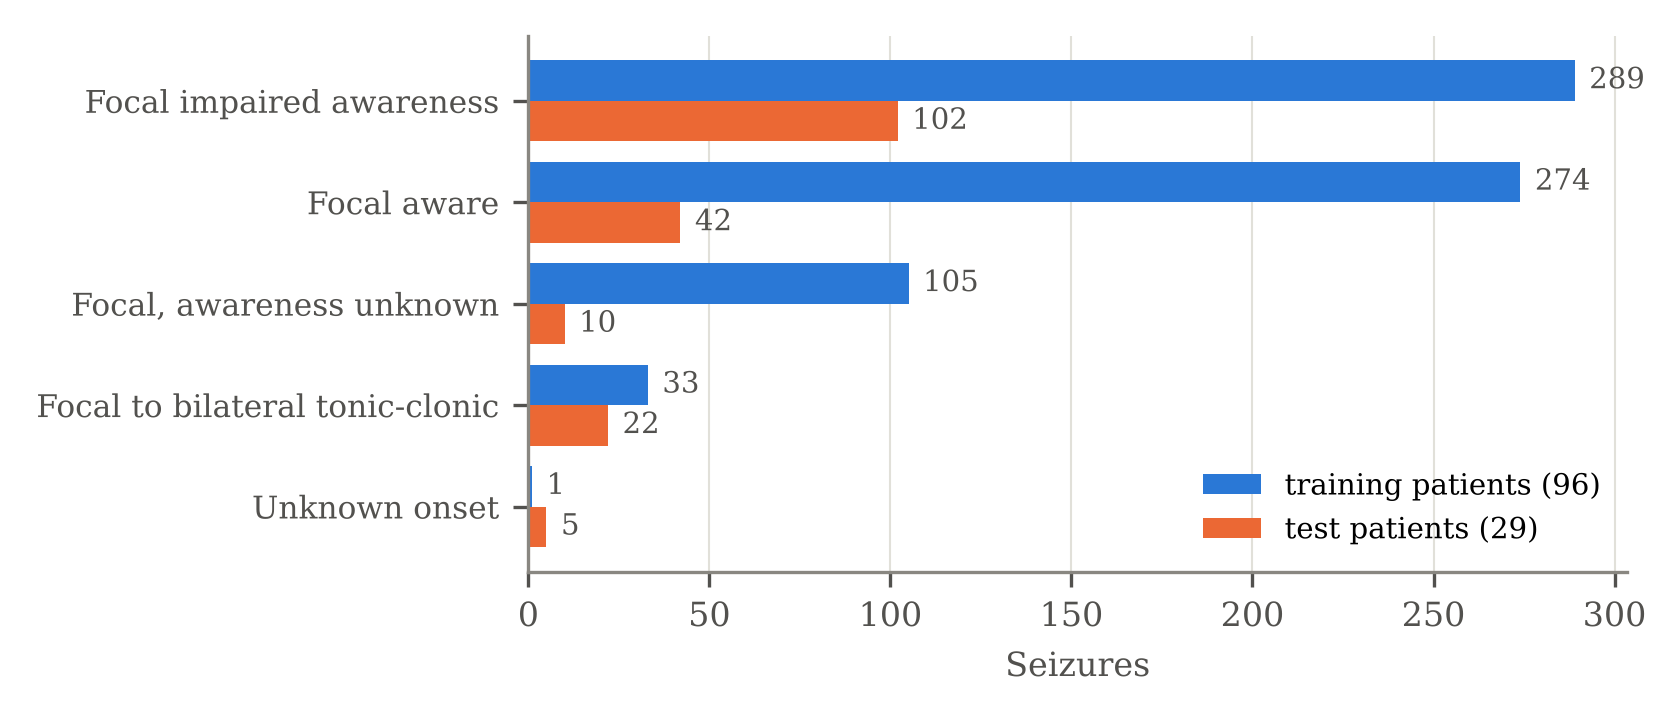
\includegraphics[width=0.78\textwidth]{figures/seizure_classes.png}
\caption{Seizure classes in the training and test patients: 822 of 883 seizures are focal seizures that do not become
tonic-clonic.}\label{fig:classes}
\end{figure}

\begin{figure}[H]
\centering
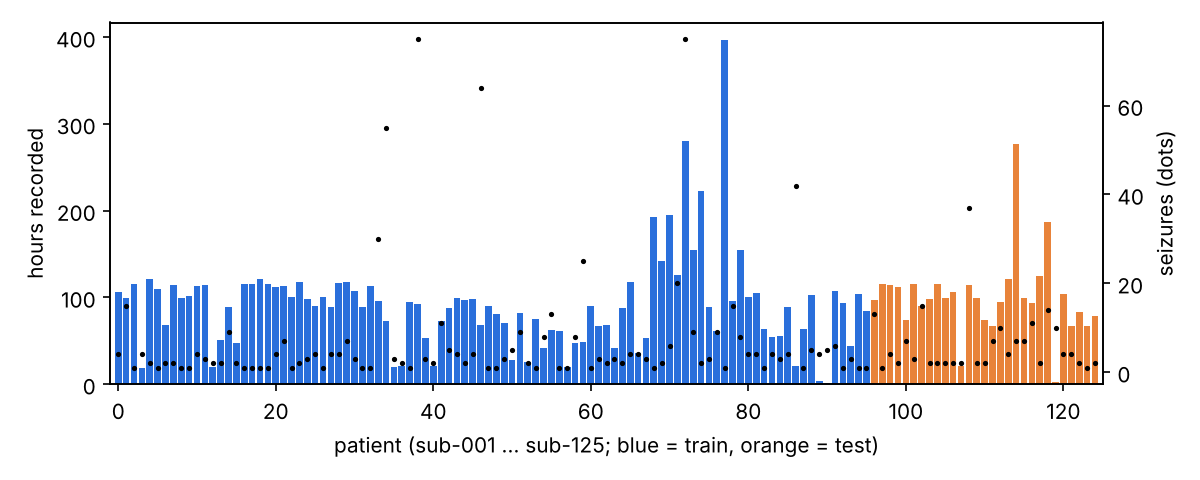
\includegraphics[width=0.9\textwidth]{figures/hours_and_seizures_per_patient.png}
\caption{Hours recorded (bars; blue: training, orange: test) and seizures per patient (dots).}\label{fig:hours}
\end{figure}

\section{Audit Findings}

\begin{table}[H]
\centering\small
\caption{Where the released files differ from the documentation, and what we did.}\label{tab:docdiff}
\begin{tabularx}{\textwidth}{@{}P{38mm}P{26mm}P{30mm}L@{}}
\toprule
\textbf{Item} & \textbf{Documentation} & \textbf{Files} & \textbf{Action}\\
\midrule
Sampling rate & 250 Hz & 256 Hz & Filters designed for 256 Hz\\
Seizures & 886 & 883 & Report our count\\
Centre and age labels & used for splits & not released & Folds by seizure count\\
Official artefact rule & 13--150\,\textmu V & flags 69\,\% of normal windows & Flags used as input bits\\
Downloads & -- & 9 files cut short & Size checks; re-extracted\\
Evaluation code & -- & two defects & Corrected values reported alongside\\
\bottomrule
\end{tabularx}
\end{table}

\section{System Architecture}

\begin{figure}[H]
\centering
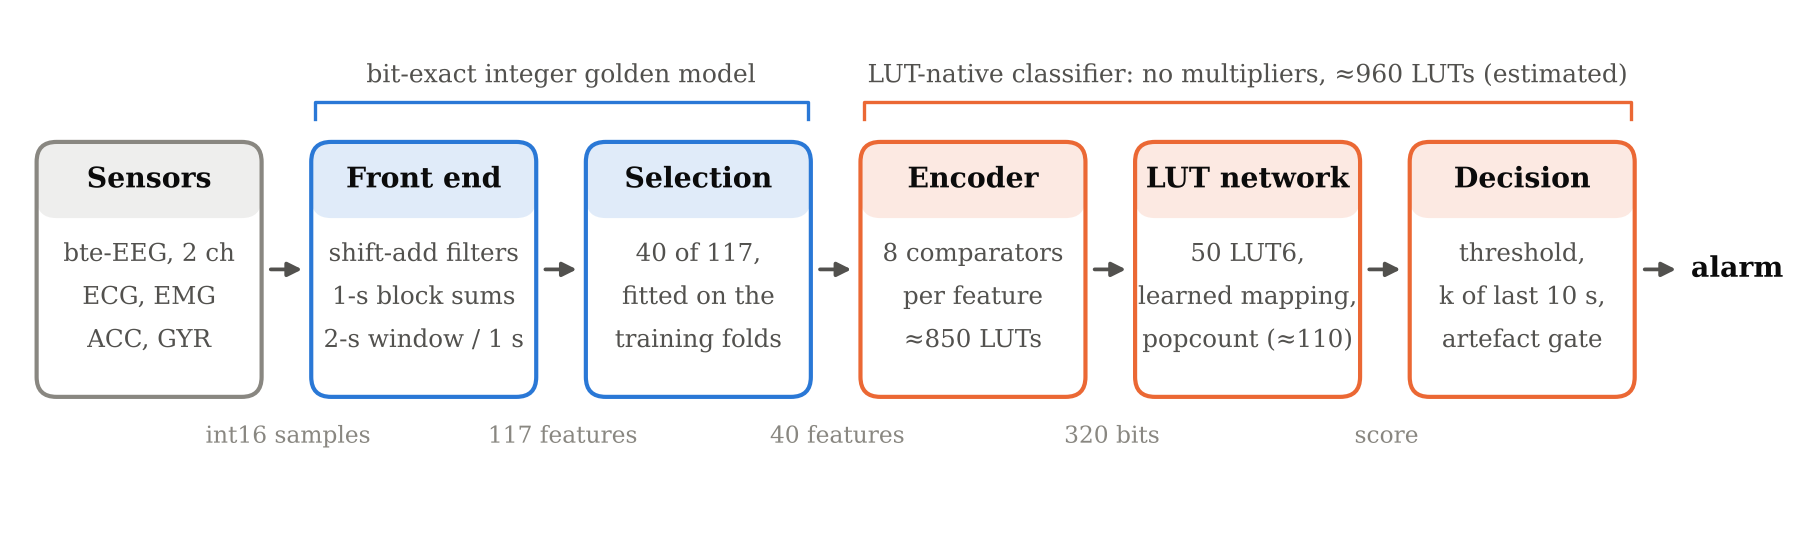
\includegraphics[width=\textwidth]{figures/system_overview.png}
\caption{The proposed detector. Blue: bit-exact integer front end; orange: LUT-native classifier.}\label{fig:system}
\end{figure}

\begin{itemize}
\item Every second, the last 2 s of all signals become \textbf{117 integer features} (Table~\ref{tab:features}).
\item The 40 most useful features are thermometer-encoded and classified by a \textbf{50-neuron LUT network}.
\item An alarm is raised when at least $k$ of the last 10 seconds are positive.
\end{itemize}

\begin{table}[H]
\centering\small
\caption{The 117 integer features (per 2-s window; many also as change from a 64-s moving average).}\label{tab:features}
\begin{tabularx}{\textwidth}{@{}lcL@{}}
\toprule
\textbf{Group} & \textbf{Count} & \textbf{Features}\\
\midrule
EEG & 84 & amplitude, line length, mobility, zero crossings, extrema, 5 band amplitudes; artefact flags\\
ECG & 5 & log heart period, log RR variability, quality flag\\
EMG & 8 & amplitude, line length, zero crossings, high/low band ratio\\
Motion & 16 & accelerometer and gyroscope magnitude, jerk, activity, band amplitude\\
Presence & 4 & one bit per sensor (ECG, EMG, accelerometer, gyroscope)\\
\bottomrule
\end{tabularx}
\end{table}

\paragraph{Integer arithmetic.} Filters use coefficients that are sums of powers of two (shifts and adds only), with
error feedback; heart rate uses $\log_2(\mathrm{RR})$, so there is no division. A floating-point twin measures the cost
of the integer arithmetic (Section~\ref{sec:intfloat}).

\section{The LUT-Native Classifier (DWN)}

A Differentiable Weightless Neural Network \cite{bacellar2024dwn} has no weights: each neuron is a 6-input truth table,
exactly one FPGA LUT.
\begin{equation}
  b_{f,i} = [\,x_f > t_{f,i}\,],\quad i = 1,\dots,8 \qquad\qquad s = \sum_{j \in S} y_j - \sum_{j \in B} y_j
\end{equation}
Each feature becomes 8 thermometer bits (one comparator each); each neuron reads 6 learned bits and outputs one stored
bit $y_j$; the score $s$ is the popcount of the seizure group $S$ minus that of the background group $B$.
Figure~\ref{fig:cost} shows the hardware cost of the final network.

\begin{figure}[H]
\centering
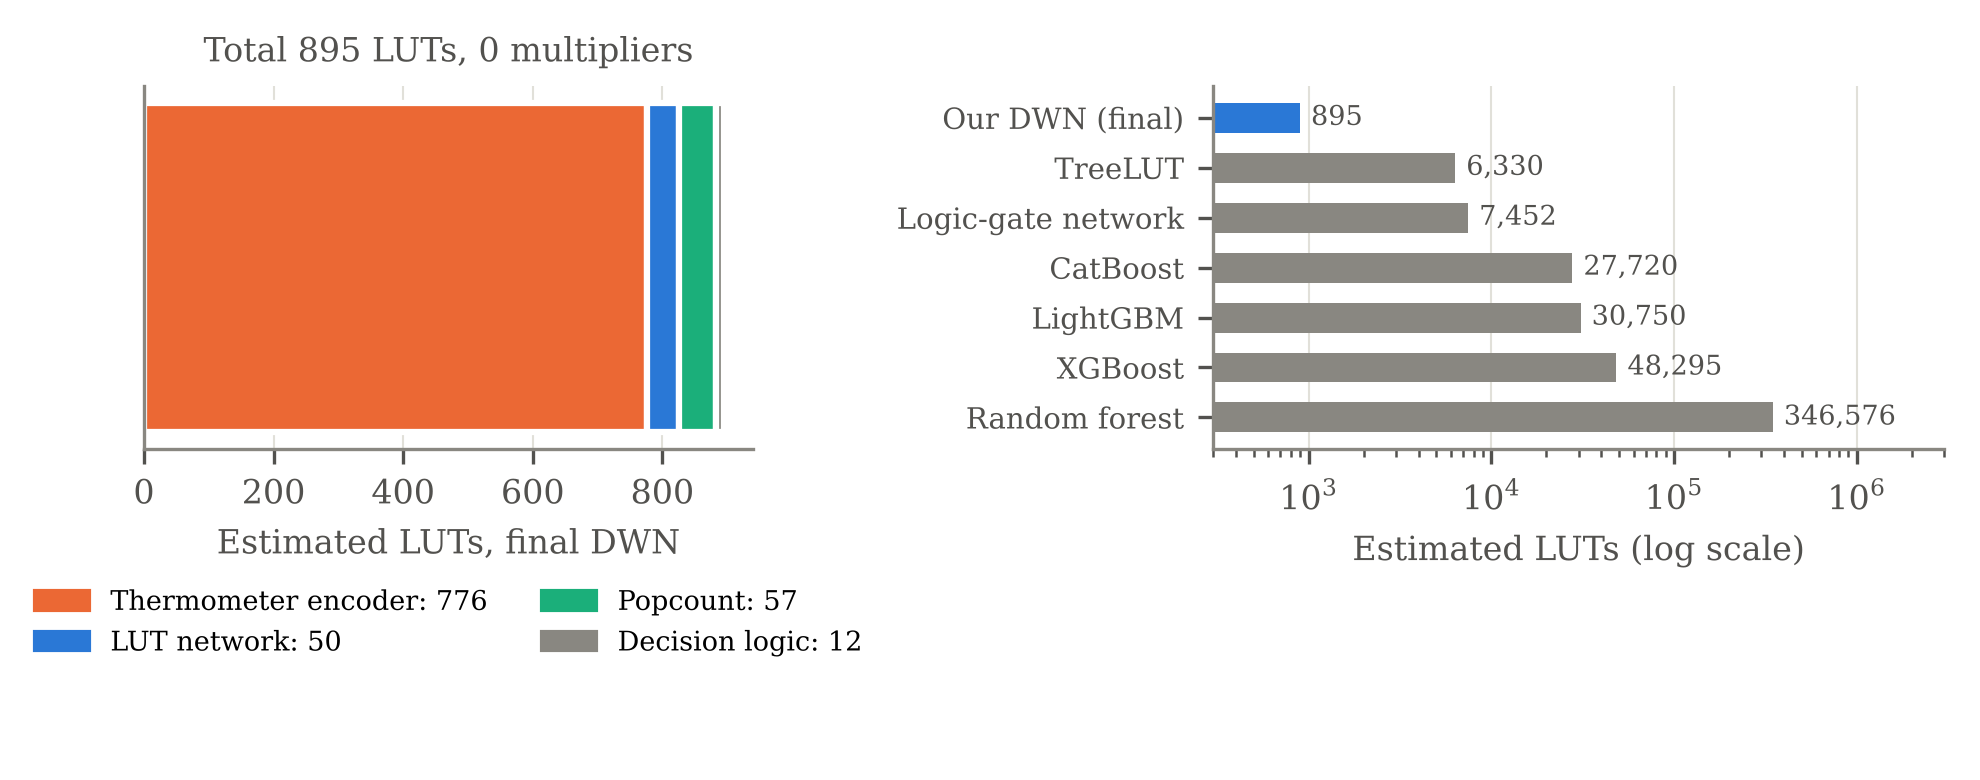
\includegraphics[width=\textwidth]{figures/cost.png}
\caption{Estimated hardware cost. Left: the final DWN by block (the encoder dominates). Right: total LUTs of each model,
log scale.}\label{fig:cost}
\end{figure}

\section{Models and Extensions}

\begin{table}[H]
\centering\small
\caption{Models compared on the same features, splits and metrics.}\label{tab:models}
\begin{tabularx}{\textwidth}{@{}P{36mm}L@{}}
\toprule
\textbf{Group} & \textbf{Models}\\
\midrule
Published baselines & ChronoNet \cite{roy2019chrononet} (CNN + GRU on raw EEG); SVM \cite{vandecasteele2020bte}\\
Software references & logistic regression, random forest, XGBoost, LightGBM, CatBoost\\
Hardware-oriented & INT8 MLP (multipliers), TreeLUT \cite{khataei2025treelut}, logic-gate network \cite{petersen2022dlgn}, DWN \cite{bacellar2024dwn}\\
\bottomrule
\end{tabularx}
\end{table}

\begin{table}[H]
\centering\small
\caption{Extensions of the DWN tested in this project (adopted only if significantly better).}\label{tab:extensions}
\begin{tabularx}{\textwidth}{@{}cL@{}}
\toprule
\textbf{ID} & \textbf{Idea}\\
\midrule
N1 & Memory across seconds: 16 state bits fed back; stacked past windows\\
N2 & Encoder design: uniform, Gaussian and learned thresholds\\
N3 & Label-free per-patient threshold adaptation\\
N4 & Distillation from LightGBM; teacher-guided hard negatives\\
N5 & Focal, noise-robust (GCE, SCE) and multiple-instance losses; onset weighting\\
N6 & Modality dropout, gated fusion, late fusion\\
N7 & Interpretability: which inputs the LUTs read during alarms\\
N8 & Post-ictal verification: a second LUT network confirms each alarm (secondary analysis)\\
\bottomrule
\end{tabularx}
\end{table}

\section{Evaluation Protocol}\label{sec:eval}

\begin{itemize}
\item \textbf{Patient-wise 5-fold cross-validation} on the 96 training patients for every design choice.
\item \textbf{Sealed test set}: the 29 test patients scored once, after the freeze, with 5 seeds; every access logged.
\item \textbf{SzCORE event scoring} \cite{dan2024szcore} (30\,s before, 60\,s after, 90\,s merge), per patient:
\end{itemize}
\begin{equation}
  \mathrm{Sens} = \frac{TP}{TP + FN},\qquad \mathrm{Prec} = \frac{TP}{TP + FP},\qquad
  F_1 = \frac{2\,\mathrm{Sens}\cdot\mathrm{Prec}}{\mathrm{Sens} + \mathrm{Prec}},\qquad \text{false alarms per 24 h}
\end{equation}
\begin{itemize}
\item \textbf{Operating points} (threshold, $k$, artefact gate) chosen on the training folds: best event-F1, and highest
  sensitivity with at most one false alarm per hour.
\item \textbf{Statistics}: paired Wilcoxon test per patient; an extension is adopted only if $p < 0.05$ in its favour.
\item \textbf{Paper metrics} (the base paper's own code) are reported for the comparison with the base paper.
\item \textbf{Compute}: a 4-core CPU server and a laptop RTX 3060 GPU.
\end{itemize}
